\documentclass[12pt]{report}
\usepackage[utf8x]{inputenc}
\usepackage{graphicx}
\usepackage{gensymb}
\usepackage{algorithm}
\usepackage[noend]{algpseudocode}
\usepackage{algpseudocode}
\graphicspath{ {./images/} }
\usepackage{fancyhdr}


\title{ETERNITY: FUNCTION}								
\author{Pragya Tomar}						
\date{}

\makeatletter
\let\thetitle\@title
\let\theauthor\@author
\let\thedate\@date
\makeatother

\pagestyle{fancy}
\fancyhf{}
\rhead{\thetitle}
\cfoot{\thepage}

\begin{document}

\begin{titlepage}
	\centering
    \vspace*{1 cm}
\begin{center}    \textsc{\Large Concordia University}\\[2.5 cm]	
{Problem 5 }\\[0.4 cm]
\end{center}
	\textsc{\Large  SOEN 6011 - Software Engineering Process }\\[1 cm]
	\rule{\linewidth}{0.5 mm} \\[0.4 cm]
	{ \huge \textbf \thetitle}\\[0.5 cm]
	{ \huge \textbf{($\sigma$)}}
	\rule{\linewidth}{0.5 mm} \\[1.0 cm]

	
\begin{center}   {\Large \textbf{\theauthor}} \\[1 cm]
                 {\large Student ID : 40197757 }\\[0.4 cm]
                 {\large Repository Address: https://github.com/pragya231/SOEN6011}
\end{center}
	
\end{titlepage}

\tableofcontents
\pagebreak

\renewcommand{\thesection}{\arabic{section}}

\section{Unit Test Cases Description}
\pagenumbering{arabic}

\subsection{Test Environment}
\begin{enumerate}
\item Eclipse IDE  for Java.
\item JUnit4 framework in Eclipse IDE for testing.
\end{enumerate}

\begin{center}
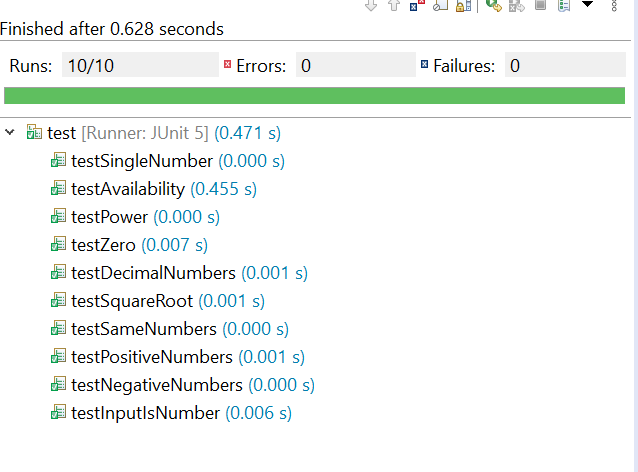
\includegraphics[width=15cm,height=6cm]{UnitTest}
\end{center}

\subsection{Descriptions}
The unit test cases for $\sigma$ function is done using Junit4 which is traceable to the requirements in Problem 2.

\textbf{Test Case : F8\_UnitTestCase\_1}\\\\
\begin{tabular}{ll}
\textbf{Test Case ID} & F8\_TestInputZero\\\\
\textbf{Requirement ID} & R1 \\
\textbf{Action} & 
\begin{tabular}[c]{@{}l@{}}The user gives an input 0 and
\\then clicks SD($\sigma$) button. \\
\end{tabular} \\
\textbf{Input(s) } & 0 \\
\textbf{Expected Output } & 0 \\
\textbf{Actual Output } &   0 \\
\textbf{Test Result } & Success \\
\end{tabular}
\\\\\\\\
\textbf{Test Case : F8\_UnitTestCase\_2}\\\\
\begin{tabular}{ll}
\textbf{Test Case ID} & F8\_TestSingleNumber\\\\
\textbf{Requirement ID} & R2 \\
\textbf{Action} & 
\begin{tabular}[c]{@{}l@{}}The user gives an input 5 and
\\then clicks SD($\sigma$) button. \\
\end{tabular} \\
\textbf{Input(s) } & 6 \\
\textbf{Expected Output } & 0 \\
\textbf{Actual Output } &   0 \\
\textbf{Test Result } & Success \\
\end{tabular}
\\\\\\\\
\textbf{Test Case : F8\_UnitTestCase\_3}\\\\
\begin{tabular}{ll}
\textbf{Test Case ID} & F8\_TestSameNumbers\\\
\textbf{Requirement ID} & R3\\
\textbf{Action} & 
\begin{tabular}[c]{@{}l@{}}The user gives an input [8 8 8 8 8] and
\\then clicks SD($\sigma$) button. \\
\end{tabular} \\
\textbf{Input(s) } & [8 8 8 8 8] \\
\textbf{Expected Output } & 0 \\
\textbf{Actual Output } &   0 \\
\textbf{Test Result } & Success \\
\end{tabular}
\\\\\\\\
\textbf{Test Case : F8\_UnitTestCase\_4}\\\\
\begin{tabular}{ll}
\textbf{Test Case ID} & F8\_TestNegativeNumbers\\\\
\textbf{Requirement ID} & R4 \\
\textbf{Action} & 
\begin{tabular}[c]{@{}l@{}}The user gives an input [-3 -7 2 -1 9] and
\\then clicks SD($\sigma$) button. \\
\end{tabular} \\
\textbf{Input(s) } & [-3 -7 2 -1 9] \\
\textbf{Expected Output } & 5.3665631459995 \\
\textbf{Actual Output } &   5.3665631459995 \\
\textbf{Test Result } & Success \\
\end{tabular}
\\\\\\\\
\textbf{Test Case : F8\_UnitTestCase\_5}\\\\
\begin{tabular}{ll}
\textbf{Test Case ID} & F8\_TestPositiveNumbers\\\\
\textbf{Requirement ID} & R5\\
\textbf{Action} & 
\begin{tabular}[c]{@{}l@{}}The user gives an input [8 6 9 10 5] and
\\then clicks SD($\sigma$) button. \\
\end{tabular} \\
\textbf{Input(s) } & [8 6 9 10 5] \\
\textbf{Expected Output } & 1.8547236990991407 \\
\textbf{Actual Output } &   1.8547236990991407 \\
\textbf{Test Result } & Success \\
\end{tabular}
\\\\\\\\
\textbf{Test Case : F8\_UnitTestCase\_6}\\\\
\begin{tabular}{ll}
\textbf{Test Case ID} & F8\_TestDecimalNumbers\\\\
\textbf{Requirement ID} & R6 \\
\textbf{Action} & 
\begin{tabular}[c]{@{}l@{}}The user gives an input [3.1 6.4 2.7 7.5 4] and
\\then clicks SD($\sigma$) button. \\
\end{tabular} \\
\textbf{Input(s) } & [3.1 6.4 2.7 7.5 4] \\
\textbf{Expected Output } & 1.8853116453255 \\
\textbf{Actual Output } &   1.8853116453255 \\
\textbf{Test Result } & Success \\
\end{tabular}
\\\\\\\\
\textbf{Test Case : F8\_UnitTestCase\_7}\\\\
\begin{tabular}{ll}
\textbf{Test Case ID} & F8\_TestSquareRoot\\\\
\textbf{Requirement ID} & R7\\
\textbf{Action} & 
\begin{tabular}[c]{@{}l@{}}Input 2 is given
to the $\sqrt{x}$ function. \\
\end{tabular} \\
\textbf{Input(s) } & 2 \\
\textbf{Expected Output } & 1.4142135623746899 \\
\textbf{Actual Output } &   1.4142135623746899\\
\textbf{Test Result } & Success \\
\end{tabular}
\\\\\\\\
\textbf{Test Case : F8\_UnitTestCase\_8}\\\\
\begin{tabular}{ll}
\textbf{Test Case ID} & F8\_TestPower\\\\
\textbf{Requirement ID} & R8 \\
\textbf{Action} & 
\begin{tabular}[c]{@{}l@{}} Input 5 as base and exponent 2 is given
\\to the power(x,y) function. \\
\end{tabular} \\
\textbf{Input(s) } & 5,2 \\
\textbf{Expected Output } & 25 \\
\textbf{Actual Output } &   25 \\
\textbf{Test Result } & Success \\
\end{tabular}
\\\\\\\\
\textbf{Test Case : F8\_UnitTestCase\_9}\\\\
\begin{tabular}{ll}
\textbf{Test Case ID} & F8\_TestInputisNumber\\\\
\textbf{Requirement ID} & R9 \\
\textbf{Action} & 
\begin{tabular}[c]{@{}l@{}}The user gives an input "g" and
then clicks SD($\sigma$) button. \\
\end{tabular} \\
\textbf{Input(s) } & "h" \\
\textbf{Expected Output } & false \\
\textbf{Actual Output } &   false \\
\textbf{Test Result } & Success \\
\end{tabular}
\\\\\\\\
\textbf{Test Case : F8\_UnitTestCase\_10}\\\\
\begin{tabular}{ll}
\textbf{Test Case ID} & F8\_TestAvailability\\\\
\textbf{Requirement ID} & R10 \\
\textbf{Action} & 
\begin{tabular}[c]{@{}l@{}}The user gives any input
then clicks SD($\sigma$) button. \\
\end{tabular} \\
\textbf{Input(s) } & Any real numbers \\
\textbf{Expected Output } & positive real number \\
\textbf{Actual Output } & positive real number \\
\textbf{Test Result } & Success \\
\end{tabular}
\\

\begin{thebibliography}{9}
    

\bibitem{ReqView} 
ReqView : Nykamp DQ: Requirements Specification Templates
\\\texttt{https://www.reqview.com/doc/iso-iec-ieee-29148-templates}
\bibitem{29148} 
29148-2018-ISO/IEC/IEEE International Standard-Systems and software engineering-Life cycle processes-Requirements engineering,
\\\texttt{https://standards.ieee.org/standard/29148-2018.html}
\end{thebibliography}




\end{document}